\documentclass[./../../paper.tex]{subfiles}
\graphicspath{{\subfix{./../../figures/}}}

\begin{document}

The \gls{damerau_levenshtein} function is a modified version of the Levenshstein distance\autocite{levenshtein_Binarycodescapable_1965}, which is a widely used to compute the edit-distance of two discrete sequences\autocites{apostolico_SequenceAlignmentMolecular_1998,Mitton20101}. The most important applications are within the \gls{NLP} discipline and the Biomedical Sciences. Within these areas, we often use the Levenshtein distance to compute the edit-distance between two words, two sentences or two DNA sequences. Note, that the elements of these sequences are often atomic symbols instead of multidimensional vectors. Generally, the distance accounts for inserts, deletions and substitutions of elements between the two serquences.
\citeauthor{damerau_techniquecomputerdetection_1964} modified the distance function to allow for transposition operations. For Process Mining, transpositions are important as one event can transition into two events that are processed in parallel and may have varying processing times\autocite{damerau_techniquecomputerdetection_1964}.
% \attention{TODO: Check how a paper describes the reason for usage} 
In \autoref{fig:dl_example}, we schematically show two sequences and their distance.





\begin{figure}[htb]
    \centering
    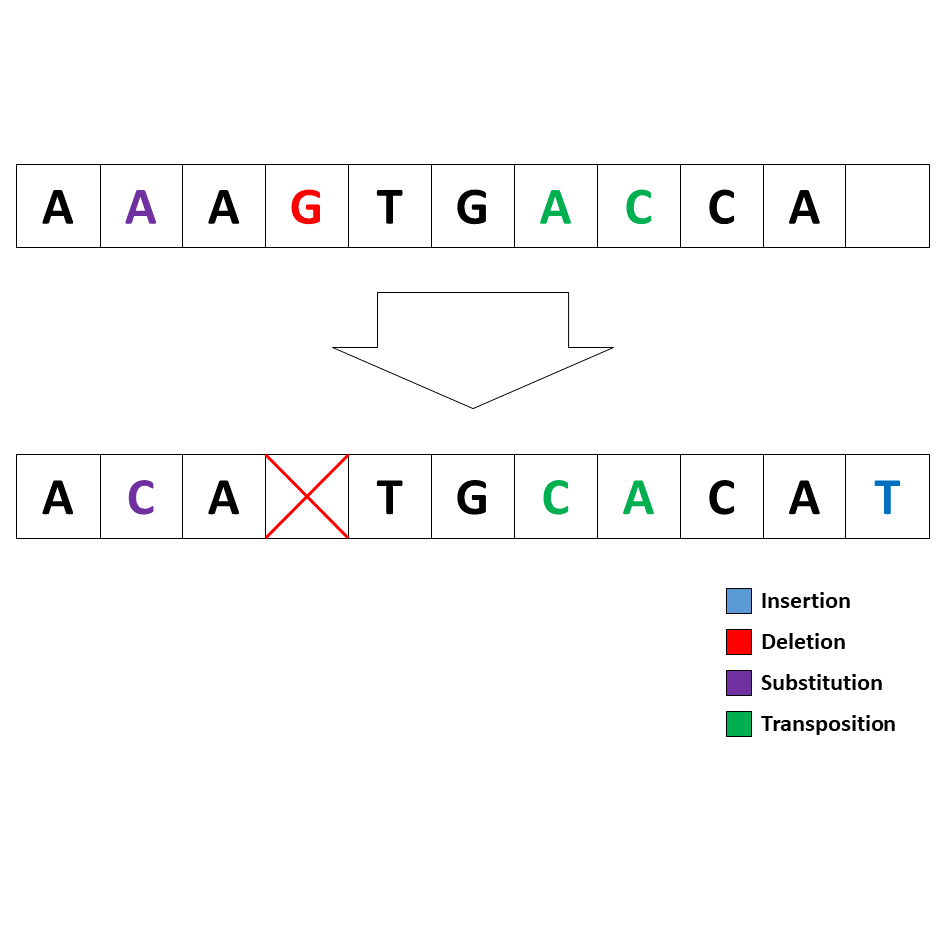
\includegraphics[width=0.75\textwidth]{figures/Graphics/Slide6.PNG}
    \caption{Two arbitrary sequences and their edit difference according to Damerau. The edit distance is the sum of each  operation necessary to transform the sequence to another sequence. Blue shows an insert, red a deletion, purple a substitution and green a transposition. Therefore, the edit distance is 4.} \label{fig:dl_example}
\end{figure}


\noindent \autoref{eq:damerau_levenshstein} depicts the recursive formulation of the distance. The distance computes the costs of transforming the sequence $a$ to $b$, by computing the minimum of five seperate terms. % TODO: change a to e for consistency with model formulation
% TODO: Read on sequence alignment literature. Also add the readup to the literature review.
\begin{align}
    \label{eq:damerau_levenshstein}
    d_{a, b}(i, j) & =\min
    \begin{cases}
        \editDistance{i-1}{j  }+ 1 & \text { if } i>0                                            \\
        \editDistance{i  }{j-1}+ 1 & \text { if } j>0                                            \\
        \editDistance{i-1}{j-1}+ 1 & \text { if } i, j>0                                         \\
        \editDistance{i-2}{j-2}+ 1 & \text { if } i, j>1 \land a_{i}=b_{j-1} \land a_{i-1}=b_{j} \\
        0                                 & \text { if } i=j=0                                         
    \end{cases}        
\end{align}

\noindent The recursive form $d_{a, b}(i, j)$ for sequences $a$ and $b$ with respective elements $i$ and $j$ takes the minimum of each allowed edit operation. In particular, no change, deletion, insertion, substitution and transposition. For each operation, the algorithm adds an edit cost of 1. 
% TODO: Change pos of no-change in listing.
% TODO: Improve flow to next section.

We cannot use the \gls{damerau_levenshtein} for process mining if the process carries additional information about event attributes. Mainly, because two events may be emitted by the same activity, but they may still carry different event attributes. 

% TODO: Change a, b and c to x, y and z or e_1, e_2 and e_3
To illustrate the issue, we explore a couple of examples. Let us assume, we have two strings $s^1=aaba$ and $s^2=acba$. Using the \gls{damerau_levenshtein}, the edit distance between both sequences is 1, as we can recognise a substitution at the second position in both strings. However, this representation is insufficient for process instances. Therefore, we now characterise the two sequences as process events rather than strings in \autoref{eq:dlexample}. 

\begin{align}
    \label{eq:dlexample}
    s^1 &=\{a,a,b,a\} \\
    s^2 &=\{a,a^*,b,a\}\\
    s^3 &=\{a,c,b,a\}\\
    s^4 &=\{a,a,b\}
    &a,b,c \in \mathbb{R}^3\\
    a &= \begin{bmatrix}
        2\\
        1\\
        4\\
    \end{bmatrix}
    a^* = \begin{bmatrix}
        3\\
        3\\
        4\\
    \end{bmatrix}
    b = \begin{bmatrix}
        1\\
        1\\
        0\\
    \end{bmatrix}
    c = \begin{bmatrix}
        3\\
        1\\
        4\\
    \end{bmatrix}
\end{align}

\noindent If we do not consider attribute values, it becomes clear that $s^2$, $s^3$ and $s^4$ have an edit-distance to $s^1$ of 0, 1 and 1. However, with attribute values in mind, $s^1$ and $s^2$ display clear differences. Similarly, $s^1$ and $s^3$ not only differ in terms of activity but also attribute value. Lastly, $s^1$ and $s^4$ are the same in attribute values, but one element still misses entirely. It appears unintuitive that each of these differences are associated with the same cost. The examples show that we can neither disregard attribute values nor events, while computing the edit distance of two \glspl{instance}. 

Instead, we have to define a cost function which takes attribute variables into account. Therefore, we modify the \gls{damerau_levenshtein} by introducing a cost function instead of a static cost. Here, the cost of each edit-type is determined by a distance-function, which considers the difference between event-attributes. Therefore, we propose an edit-function, which captures structural sequence differences, as well as, content related differences. Going back to our example, if assume our cost function to only count differences in attributes, then the difference between $s^1$ and $s^2$ shall be 2 as their activities are the same, but the first two event attributes are different. To illustrate the structural elements, the difference between $s^1$ and $s^3$ shall be 3 instead of 2. Even if both $a$ and $c$ have two common event attributes, the activities they represent are still different. For instance, if both $s^1$ and $s^3$ were medical processes and $a$ and $c$ represented taking a cancer drug or a placebo, anyone would understand both activities are different even if the patient took the same dosage.

% # TODO: This is hard to understand

\end{document}